\section{Results}

\subsection{Residual Map of an IRAC Image}
We produced a residual map for a $\sim 8$ acrsecond$^2$ region in the IRAC $ch1$ telescope image. We adopted the model-based photometry method described in section 2.1.2 for creating intrinsic light profiles of sources. The parameters used for the Sérsic profiles were extracted by Farmer from the optical-NIR images of COSMOS2020 and then included in the catalogue and the PSF for the IRAC camera \textcolor{blue}{reference} was used for convolution. In total we detected 9500 sources in the image and modelled 7173 of them, the vast majority of them being point source galaxies. The number of sources modelled with each profile type is reported in table \ref{Models_stat}. Here we also report the number of objects we had to remove from the modelling process due to unphysical parameters. Examples of the unphysical parameters include negative fluxes, effective radii of zero extent (in the models using this parameter) or axis ratios above 10, which produced unusually elliptical galaxies appearing as narrow elongated lines. The number of flagged objects that were modelled is also reported. %These are the models where the fitting in the Farmer tool did not converge. \\
\begin{table}[]
\begin{centering}
\begin{tabular}{lllll}
\hline
\textbf{Model type} & \begin{tabular}[c]{@{}l@{}}Total number \\ of sources\end{tabular} & \begin{tabular}[c]{@{}l@{}}Number of removed \\ sources due to \\ illogical parameters\end{tabular} & \begin{tabular}[c]{@{}l@{}}Number of \\ sources modelled\end{tabular} & \begin{tabular}[c]{@{}l@{}}Number of \\ flagged objects\\ (of those that \\ are modelled)\end{tabular} \\ \hline
Point Source & 6844 & 1635 & 5209 & 69 \\
Simple & 188 & 57 & 131 & 6 \\
Exponential & 1782 & 432 & 1350 & 17 \\
De Vaucouleur & 517 & 198 & 319 & 17 \\
Composite & 169 & 5 & 164 & 0 \\ \hline
\textbf{Sum} & 9500 & 2327 & 7173 & 109 \\ \hline
\end{tabular}
\end{centering}
\caption{Overview of the number of sources modelled in tile 7-7 of the IRAC ch1 telescope image with parameters extracted from Farmer. Columns from left to right: (1) The model type used, (2) Total number of detected sources, (3) Number of objects that had to be removed when performing a sanity check, (4) Number of sources left, that were actually modelled, (5) The number of objects that were modelled even though the fitting process in Farmer failed to converge.}
\label{Models_stat}
\end{table}

\begin{figure}[h!]
    \centering
    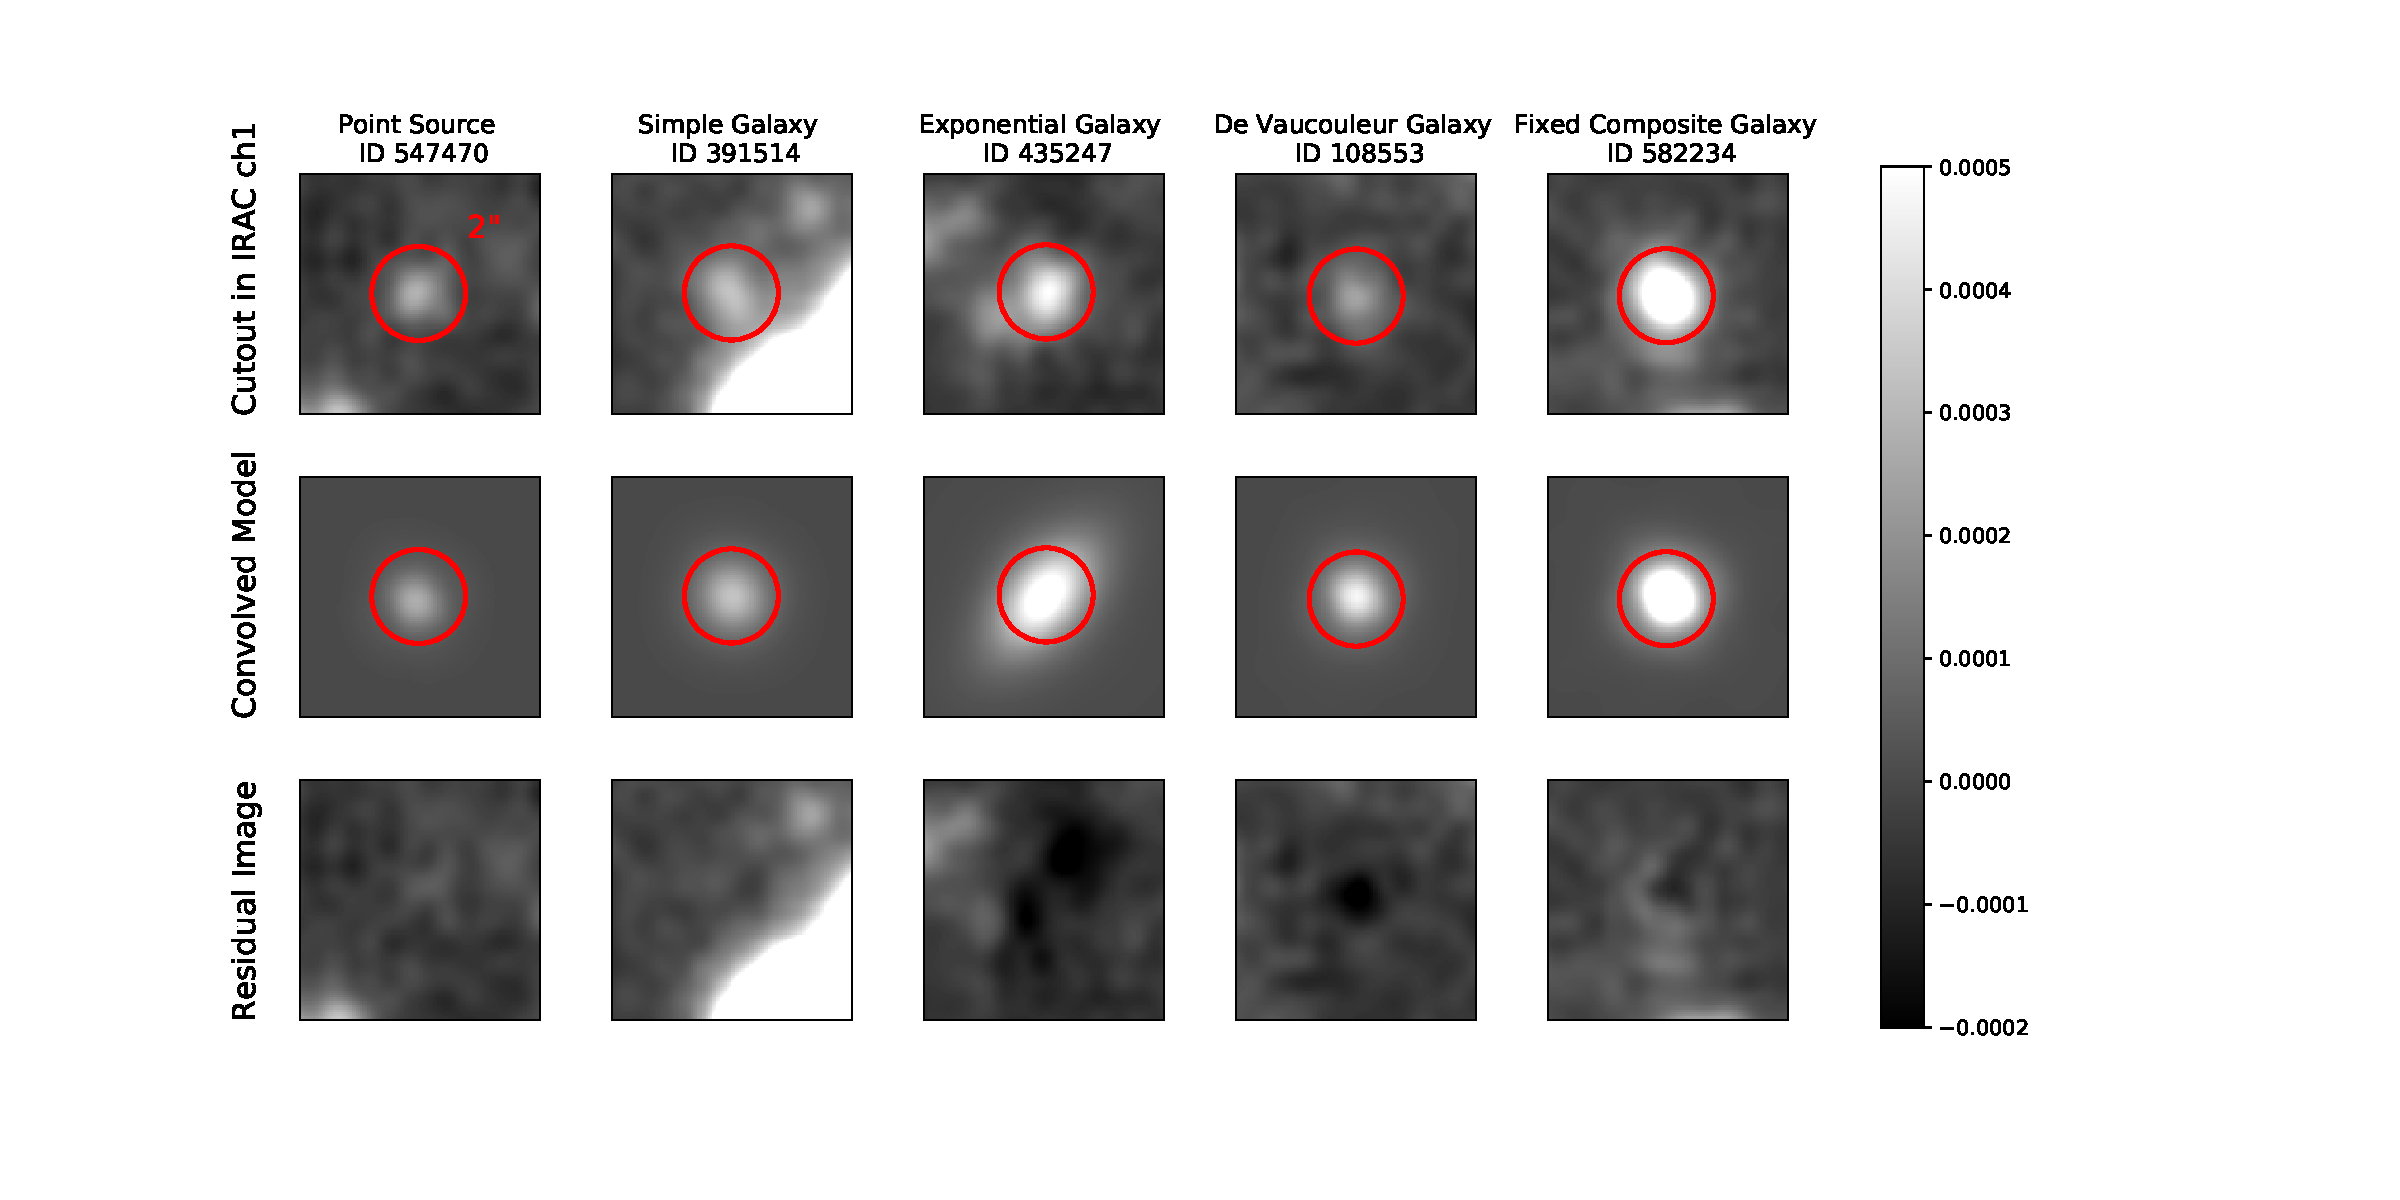
\includegraphics[trim={3cm 2.5cm 5cm 1.5cm},clip,scale=0.5]{Code/Saved_Figures/Model_cutouts.pdf}
    \caption{A good example of source modelling, for each of the five Farmer model types. The first row displays a cutout from the telescope image. The intrinsic profiles, are convolved with the IRAC PSF in the second row. The bottom row displays the residual computed by subtracting the second row from the first.}
    \label{Model_cutouts}
\end{figure}

\begin{wrapfigure}{r}{0.4\textwidth}
    \centering %left, lower, right, upper
    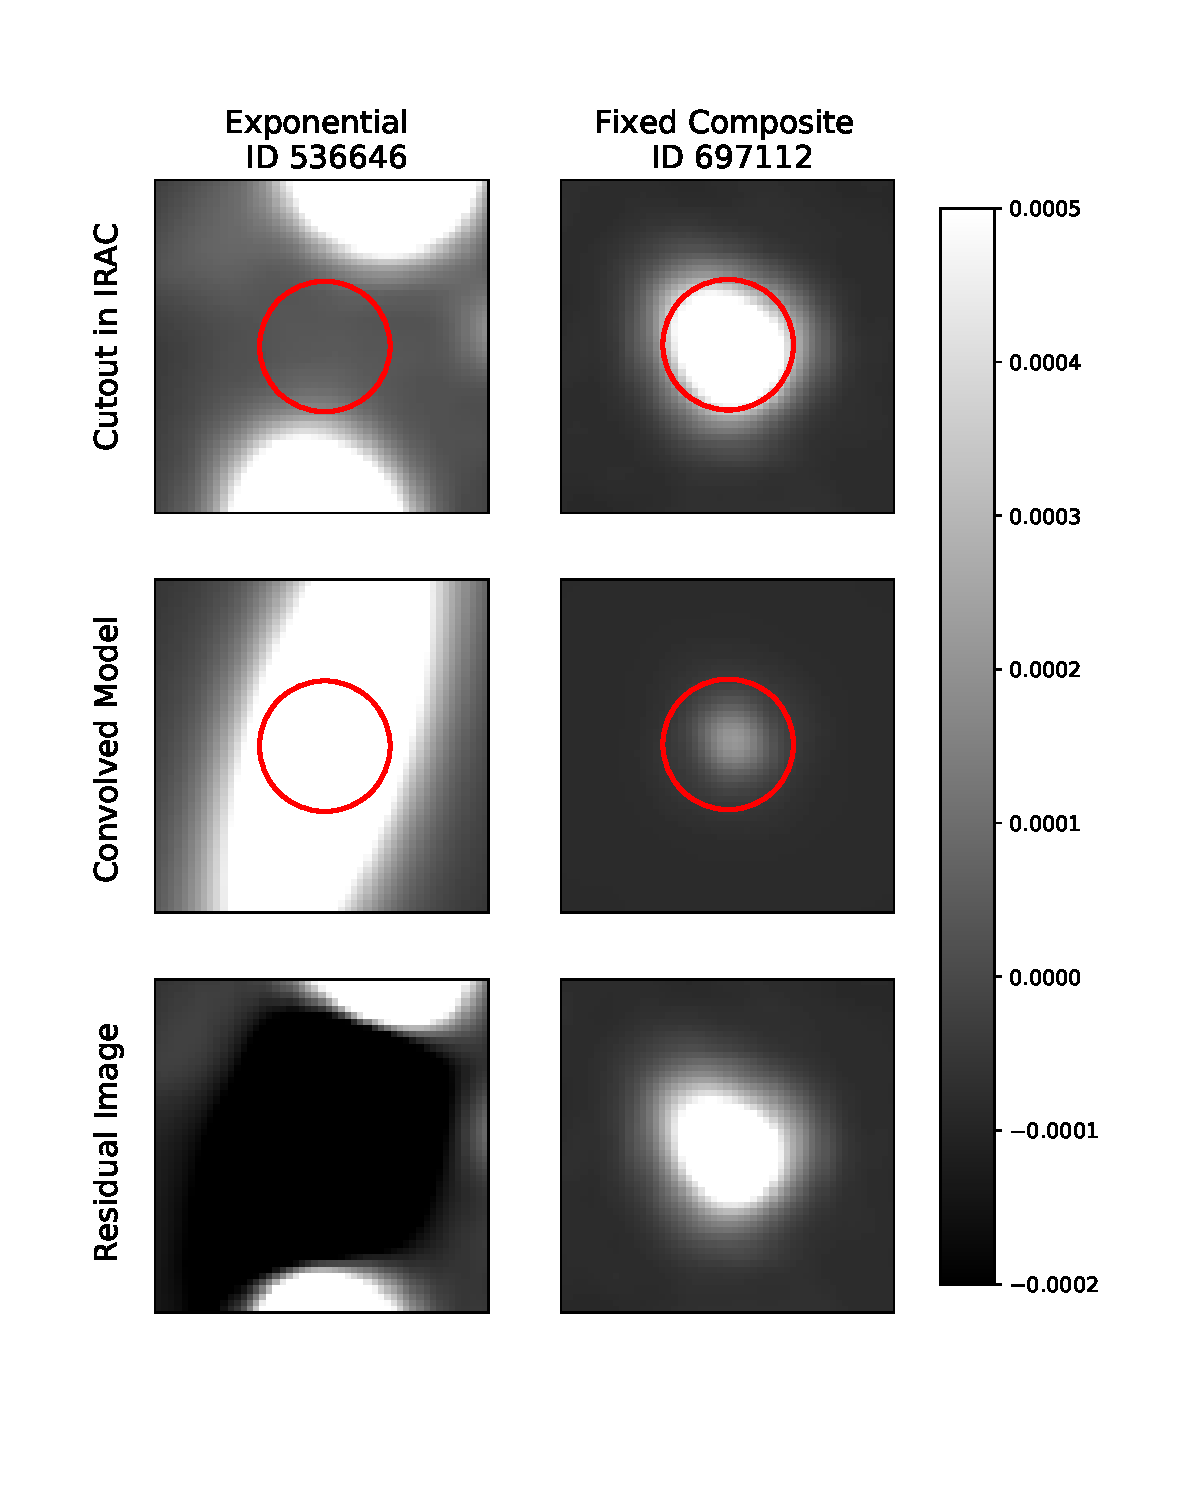
\includegraphics[trim={1cm 2.5cm 2cm 1.5cm},clip,width=0.38\textwidth]{Code/Saved_Figures/BAD_model_cutouts.pdf}
    \caption{\textcolor{blue}{write caption}}
    \label{Two examples where the modelling of the sources was not as succesful.}  
\end{wrapfigure}

We produced a combined model image, only including the sources (not the background), and placing the centre of each source model at the centroid coordinates reported in the COSMOS 2020 Classic catalogue. A $1\times1$ arcmin$^2$ section of the resulting residual image is displayed alongside the same region in the telescope image in fig.~\ref{Comparing_residual_maps} in the appendix \textcolor{blue}{change plot, github is not working due to an update so will be changed soon}. An example where the modelling performed well and produced a good residual, for each model type, is displayed in fig.~\ref{Model_cutouts}. Similarly, two examples, where the profile-fitting did not perform well, are displayed in fig.~\ref{BAD_Model_cutouts}.

\subsection{Dimensionality Reduction}
Performing source detection with SEP on an IRAC residual map, we identify 3139 objects. We used the classic residual map (described in section 2.1.1), since we did not have time, nor computational power, to produce an IRAC-size robust residual map. Furthermore a few problems arose in the residual map that was created following the description in section 2.1.2 (this is discussed in section 4). 

A residual catalogue is created, containing  information about the detected sources from telescope images (cutouts of 21$\times$21 pixels corresponding to 3.15''$\times$3.15'') in four bands: $H$, $Ks$, $ch1$ and $ch2$. These cutouts are used as the input for the t-SNE method, described in section 2.2.1 to create a 2d embedding of the higher dimensional space (21$\times$21$\times$4) in which each object is represented. To select an appropriate perplexity value, the embedding is computed for multiple values of the hyper parameter. The embedding results, from all perplexities explored, are displayed in fig. \ref{embeddding_H_ks}, \ref{embeddding_ks_ch1}, and \ref{embeddding_ch1_ch2} in the appendix, where the colours between each consecutive band are mapped. In fig. \ref{SMALL_embeddding_ks_ch1} a few select embeddings are plotted. Here the colour $Ks-ch1$ is used to colour map the sample, since this is where we search for dropouts. The colour is defined as the difference in magnitude between two bands \footnote{reference to MBW book}. Due to negative flux values, the magnitudes are sometimes undefined. These objects are assigned another colour in the plot, depending on which band the problem occurred in, so as to be able to distinguish them from the non problematic cases. We chose to continue with a perplexity of 40, since it is in the suggested range between 1 and 50 and it produces a useful clustering with a well separated cluster to the right. Furthermore the embedding was obtained with 6349 iterations which is lower than the maximum number of iterations set to 1000, hence the method has converged.
\begin{figure}[]
    \centering %left, lower, right, upper
    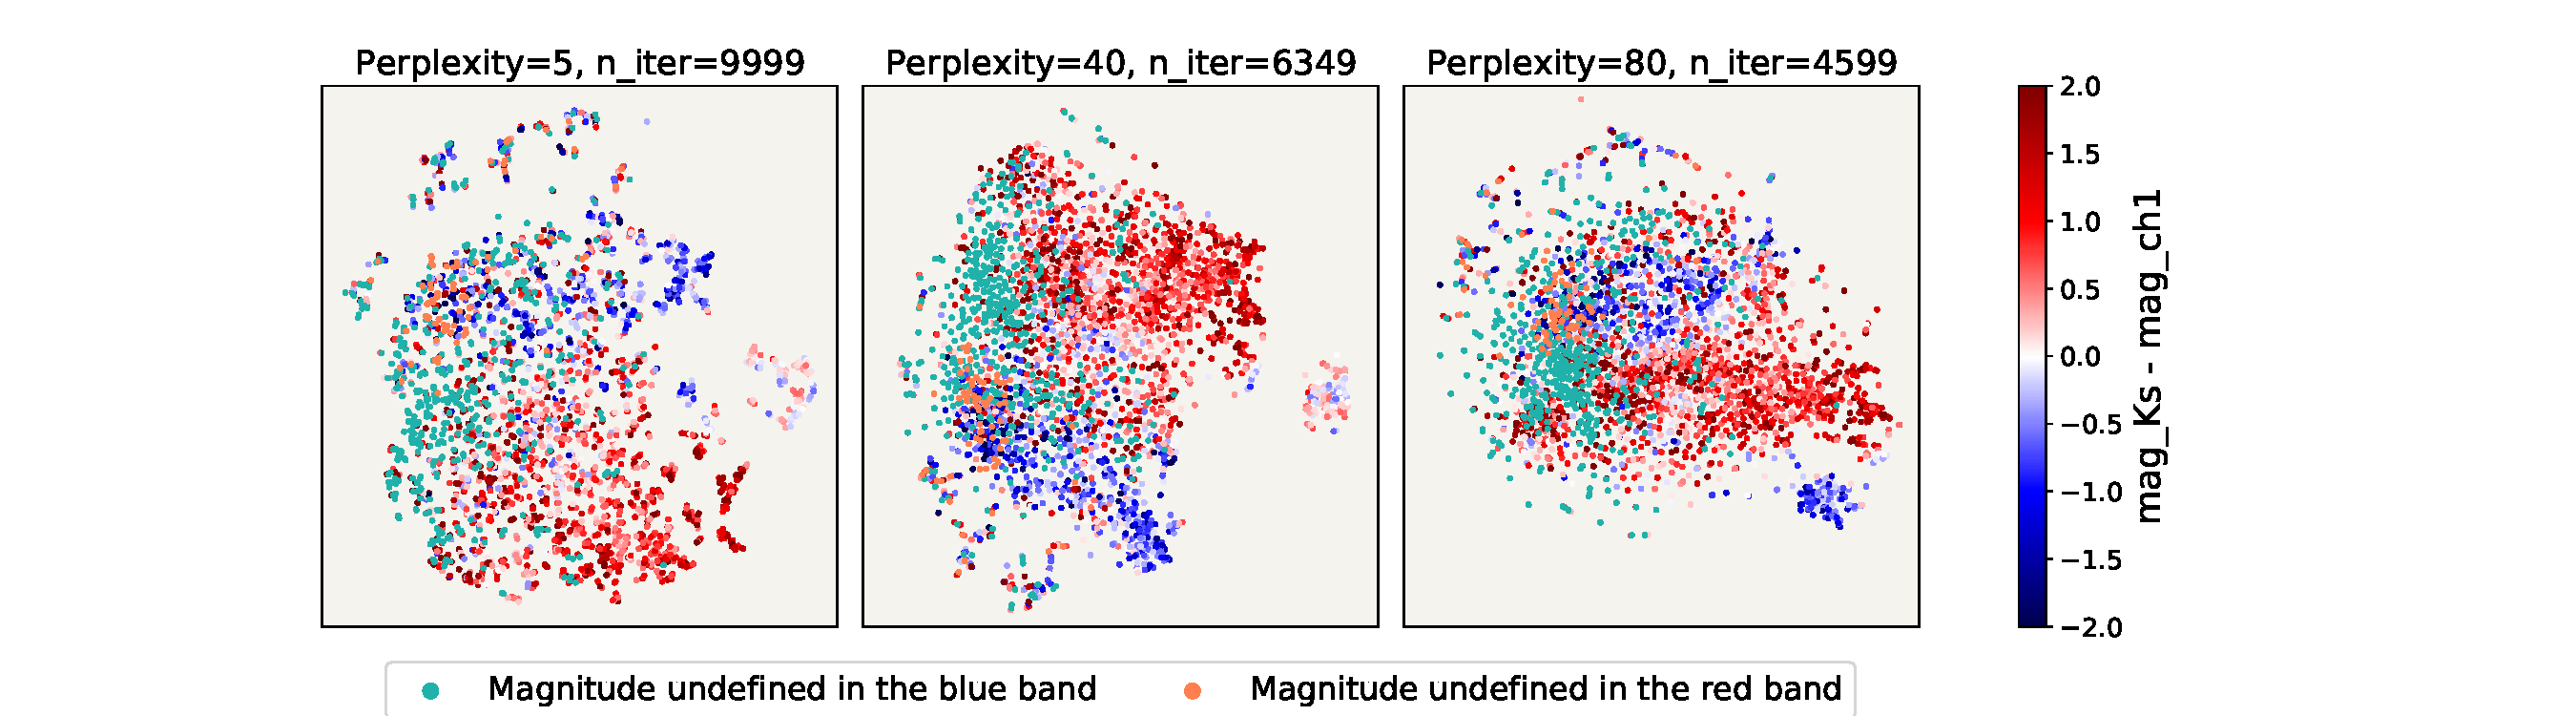
\includegraphics[trim={5cm 0cm 5cm 0.5cm},clip,width=\textwidth]{Code/Saved_Figures/peplex_Ks_ch1_SMALL.pdf}
    \caption{The t-SNE embedding results for three different perplexities. All embedding has a maximum number of iterations set to 1000. $n_iter$ reports the number of iterations actually used.}
    \label{SMALL_embeddding_ks_ch1}
\end{figure}

From manual visual inspection of the four bands, we labelled the best tracers of NIR dropouts. Furthermore we matched the coordinates of the detected objects in the residual map with the coordinates from the sources in the COSMOS 2020 Classic catalogue, to identify detection due to leftover flux in the residual map. The dense cluster located to the right in the middle plot in fig. \ref{SMALL_embeddding_ks_ch1}, is also explored, and mapping the fluxes we find that these are particular bright sources. In fig. \ref{embedding_regions} these regions are explored by plotting a cutouts from objects in each region. This figure also shows the cutouts for an object that was mapped far away from the others, it is however deemed to be of no interest for our purpose.

\begin{figure}[]
    \centering %left, lower, right, upper
    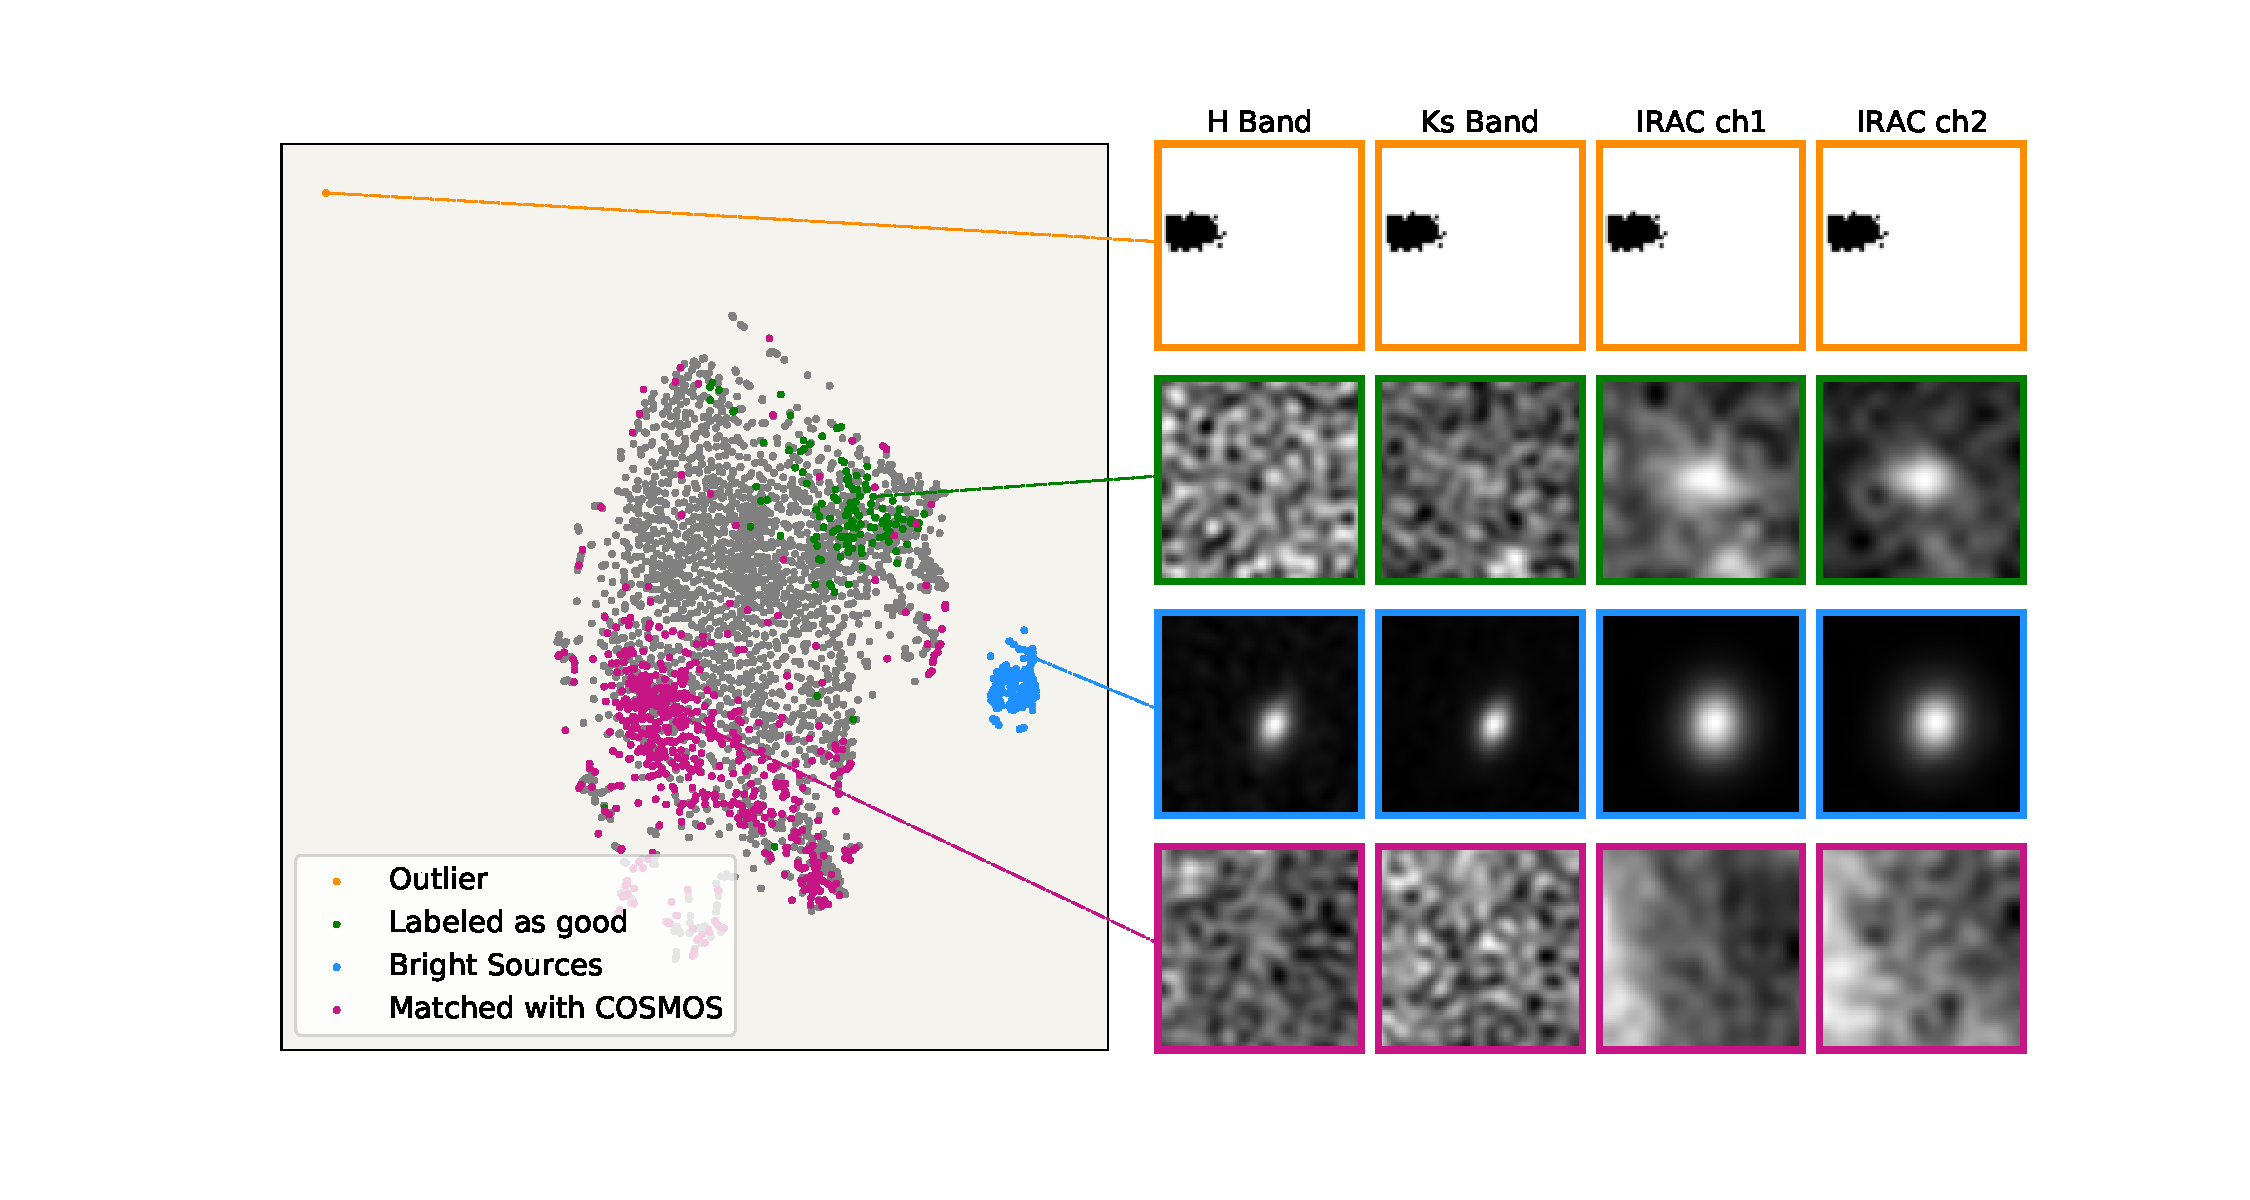
\includegraphics[trim={0cm 0cm 0cm 0cm},clip,width=\textwidth]{Code/Saved_Figures/Visual_inspection_embedding.pdf}
    \caption{The main plot shows the t-SNE embedding for perplexity 40, where objects in different regions are marked. The telescope images of an object in each region is also plotted, where the colourbar is restrained to the minimum and maximum flux detected for the object shown from the tracer region.}
    \label{embedding_regions}
\end{figure}

\subsection{Predictions}
To produce predictions and perform validation, we split all the labelled objects (including tracers) into two sets. In total we use 1069 objects labelled as non NIR-dropouts and 133 tracers. To produce predictions, respectively 1025 and 90 non dropouts and tracers are used, while respectively 44 and 43 are used for validation of the method. The validation sample is selected so it balances the two possible outputs. We ran the classification code on the training sample, which in addition to the labelled objects also includes unknown objects, with $k=15$ neighbours and 100 values of $f_{min}$ between 0 and 1, producing the results displayed in the first two left plots in fig. \ref{classification_plot}. The purity of the NIR dropout predictions was computed for each run of the classification. The parameters $f_{min}=0.47$ and $k=15$ produced the highest purity, found to be 86\%, and was therefore selected to produce the predictions displayed in the far right plot in fig.~\ref{classification_plot}. \\

To inspect the results we plot the SED of the predicted NIR-dropouts, shown in fig.~\ref{SED}. For comparison of different regions in the embedding, the SED for respectively the matched and bright objects shown in fig.~\ref{embedding_regions} are also shown.

\begin{figure}[]
    \centering %left, lower, right, upper
    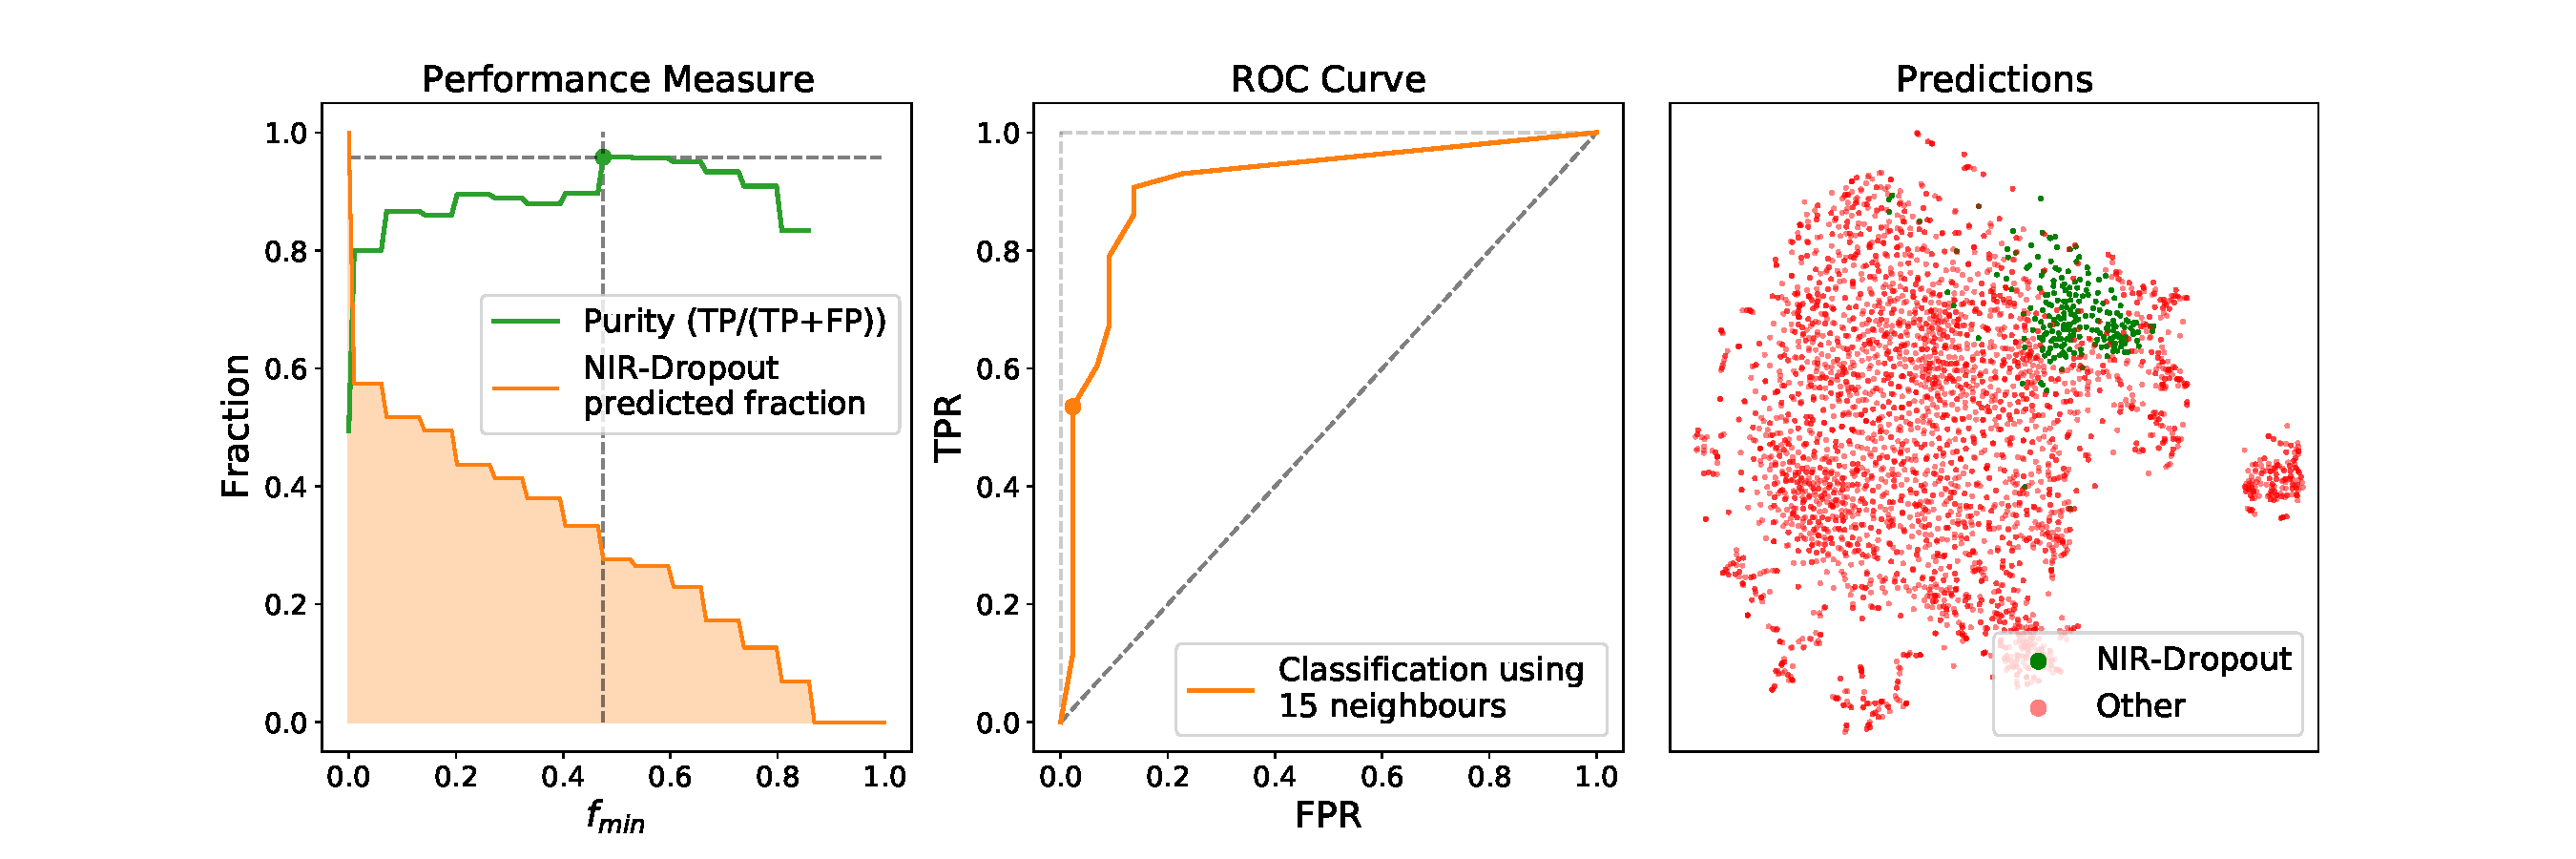
\includegraphics[trim={3.5cm 0cm 4.5cm 0cm},clip,width=\textwidth]{Code/Saved_Figures/Classification_plot.pdf}
    \caption{From left to right: (1) Performance measure as a function of the threshold $f_{min}$. In green the purity is plotted defined as the number of true positive (TP) divided by the number of total number of predicted positives (TP+FP) where FP is the number of false positives. The maximum purity achieved is marked with a green dot. (2) The receiver operating characteristic (ROC) curve. The value of $f_{min}$ corresponding to the maximum purity is marked with an orange dot. (3) The predictions produced with $f_{min}=0.47$ and $k=15$ which lead to the highest purity.}
    \label{classification_plot}
\end{figure}

\begin{figure}[]
    \centering %left, lower, right, upper
    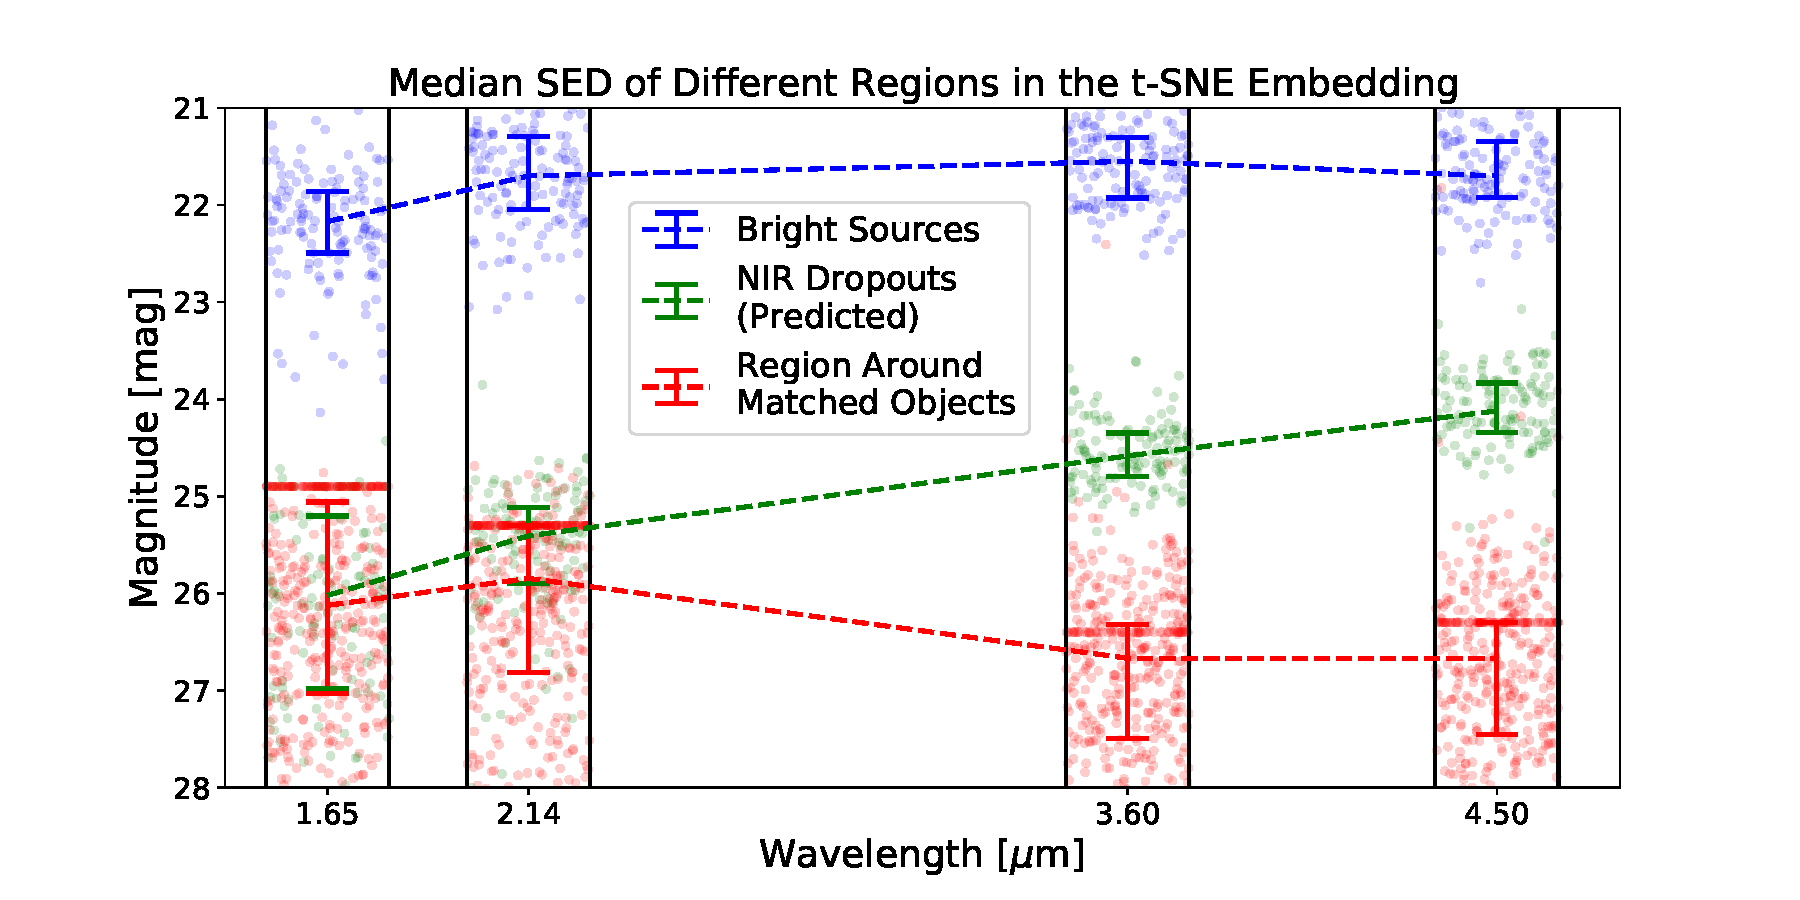
\includegraphics[trim={1cm 0cm 1cm 0cm},clip,width=\textwidth]{Code/Saved_Figures/SED_plot.pdf}
    \caption{Spectral energy distribution for objects that are found in the bright source region (blue), objects in the densest regions of sources matched with the COSMOS 2020 Classic catalogue (red) and objects that are predicted to be NIR-dropouts (green). \textcolor{blue}{nan values are replaced with upper limits from johns article}}
    \label{SED}
\end{figure}
